\documentclass[]{article}

\usepackage[margin=1.0in]{geometry}

\usepackage{amsmath}  % assumes amsmath package installed
\usepackage{amssymb}  % assumes amsmath package installed
\usepackage{graphicx}
\usepackage{todonotes}
\usepackage{float}
\usepackage{lipsum}

\usepackage[framed,numbered,autolinebreaks,useliterate]{mcode}
%\usepackage{filecontents}
\usepackage{pdfpages}

% for subfigures
\usepackage{caption}
\usepackage{subcaption}

%
%opening
\title{Probabilistic Algorithms for Aerospace Autonomy\\ASEN 6519 - Homework 1\\Inference on Hidden Markov Models}
\author{Carl Stahoviak}

\begin{document}

\maketitle

%\begin{abstract}
%
%\end{abstract}

\tableofcontents
%\listoftodos[Notes]

\newpage
\section*{Problem 1 - Forward-Backward Algorithm}
\addcontentsline{toc}{section}{Problem 1 - Forward-Backward Algorithm, Short Sequence}

Implement the forward-backward algorithm for the \texttt{nominal\_hmm\_short\_log.txt} sequence. Report the posterior probabilities $P(x_k \vert y_{1:T})$ for each timestep $k$.

\begin{table}[ht]
	\caption{Posterior Probabilities, $P(x_k \vert y_{1:T})$} 	% title of Table
	\centering 										% used for centering table
	\begin{tabular}{c c c c c} 						% centered columns (5 columns)
		\hline\hline 								%inserts double horizontal lines
		timestep, $k$ & $P(x_k = x_1 \vert y_{1:T})$ & $P(x_k = x_2 \vert y_{1:T})$ & $P(x_k = x_3 \vert y_{1:T})$ & $P(x_k = x_4 \vert y_{1:T})$ \\ [0.5ex] % inserts table
		%heading
		\hline 										% inserts single horizontal line
		1  & 0      & 0.9512 & 0.0487 & 0 \\ 		% inserting body of the table
		2  & 0      & 0.0123 & 0.9877 & 0 \\
		3  & 0      & 0.1538 & 0.8462 & 0 \\
		4  & 0      & 0.1057 & 0.8943 & 0 \\
		5  & 0      & 0.8982 & 0.1018 & 0 \\ 
		6  & 0      & 0.0022 & 0.9978 & 0 \\ 
		7  & 0      & 0.9418 & 0.0582 & 0 \\
		8  & 0.1833 & 0      & 0      & 0.8167 \\
		9  & 0.0100 & 0      & 0      & 0.9900 \\
		10 & 0.9768 & 0      & 0      & 0.0232 \\
		11 & 0.0012 & 0      & 0      & 0.9988 \\
		12 & 0.9310 & 0      & 0      & 0.0690 \\
		13 & 0.0023 &  0     & 0      & 0.9977 \\ 
		14 & 0.9509 & 0      & 0      & 0.0491 \\
		15 & 0.0549 & 0      & 0      & 0.9451 \\ [1ex]	% [1ex] adds vertical space							
		\hline 								% inserts single line
	\end{tabular}
	\label{table:posterior} 				% is used to refer this table in the text
\end{table}

\noindent Report the data log-likelihood $\log P(y_{1:T})$ for all $T$ observations. Starting with the definition of $\alpha(x_k)$, we have $\alpha(x_k) = P(x_k, \: y_{1:k})$. At the final timestep $T$, we have $\alpha(x_T) = P(x_T, \: y_{1:T})$. Marginalizing over $x_T$ gives the data likelihood $P(y_{1:T})$

\begin{equation}
	P(y_{1:T}) = \sum_{x_T} P(x_T,\: y_{1:T}) = \sum_{x_T} \alpha(x_T) = \sum_{i=1}^n \alpha_i(x_T)
\end{equation}

where $n$ is the number of discrete states. And thus the data \emph{log}-likelihood, can be written as:

\begin{equation}
	\log P(y_{1:T}) = \log \sum_{x_T} \alpha(x_T) = -28.138526
\end{equation}

\noindent Use the resulting posterior $P(x_k \vert y_{1:T})$ to classify the most likely state $x_k$ for each timestep $k=1:T$ (plot these as a time trace).

 
\begin{figure}[H]
	\begin{center}  
		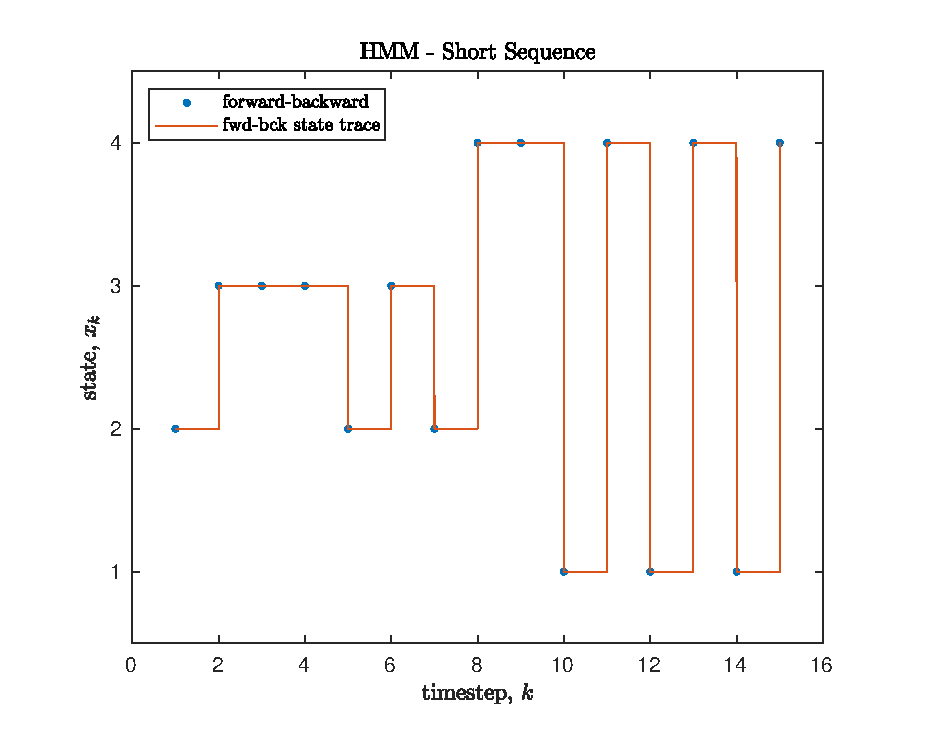
\includegraphics[scale=0.49]{p1_state_trace.eps}  
		\caption{Forward-Backward Algorithm state trace - Short Sequence}
		\label{fig:short_fb}
	\end{center}  
\end{figure}

\section*{Problem 2 - Likelihood-Weighted Approximate Inference}
\addcontentsline{toc}{section}{Problem 2 - Likelihood-Weighted Approximate Inference, Short Sequence}

The posterior $P(x_k \vert y_{1:T})$ can be constructed from the Monte Carlo sample sequences as follows

\begin{equation}
	P(x_k = x_i \vert y_{1:T}) = \frac{\sum_{s=1}^{Ns} w_s \cdot \text{ind}(x_k = x_i)}{\sum_{s=1}^{Ns} w_s}
\end{equation}

where $w_s$ is the Monte Carlo sequence weight generated according to Algorithm 2.5 in Kochenderfer, and $\text{ind}()$ is the indicator function, and simply returns one when $x_k = x_i$.\\

For Monte Carlo samples sizes $N_s$ of 100, 1000 and 10,000 the following results are achieved. Each MC sample sequence is a sequence of discrete states chosen randomly according to the state transition probability table, $P(x_k \vert x_{k-1})$. For sample sizes of less than 10,000 samples, the results (the predicted discrete states) of the likelihood-weighted approximate inference method are unreliable. Given a sample size of 10,000 or greater, the likelihood-weighted approximate inference agrees with the forward-backward algorithm.

\begin{figure}[H]
	\begin{subfigure}[b]{0.45\textwidth}
		\begin{center}  
			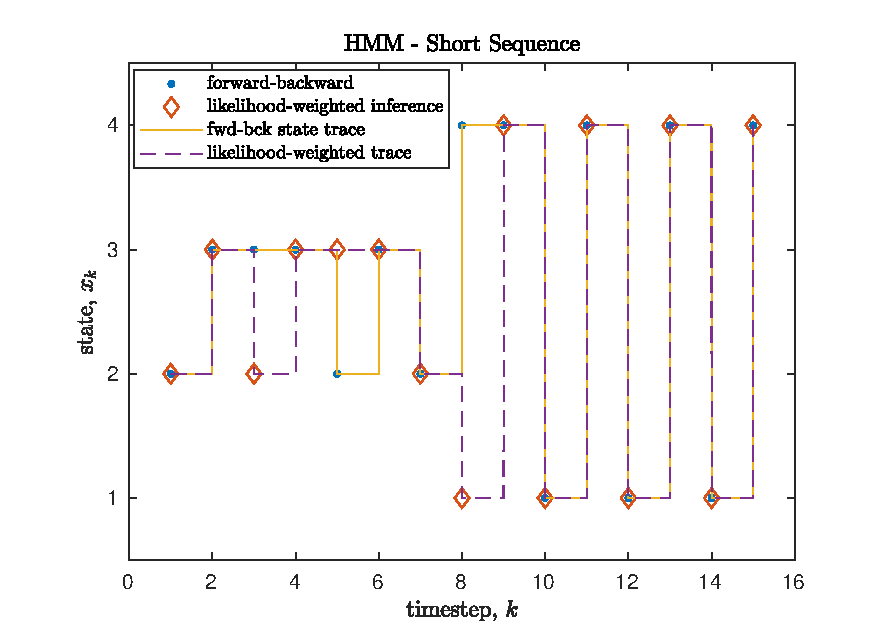
\includegraphics[scale=0.55]{p2_state_trace_100_1.eps}  
			\caption{}
			\label{}
		\end{center}
	\end{subfigure}
	\hfill
	\begin{subfigure}[b]{0.45\textwidth}
		\begin{center}  
			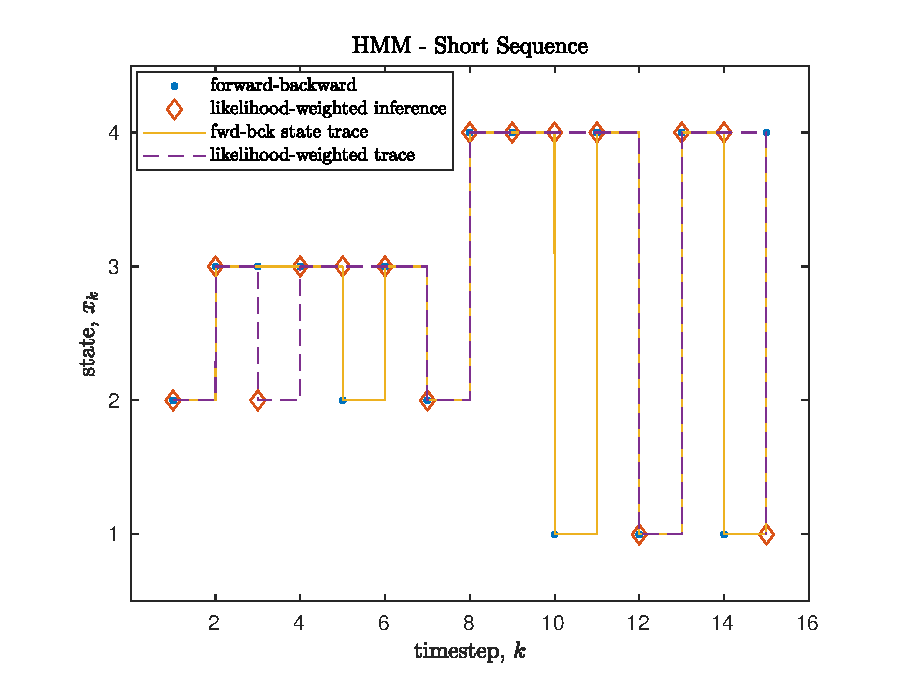
\includegraphics[scale=0.55]{p2_state_trace_100_2.eps}  
			\caption{}
			\label{}
		\end{center}
	\end{subfigure}
	\caption{Monte Carlo sample size, $N_s$ = 100}
\end{figure}

\begin{figure}[H]
	\begin{subfigure}[b]{0.45\textwidth}
		\begin{center}  
			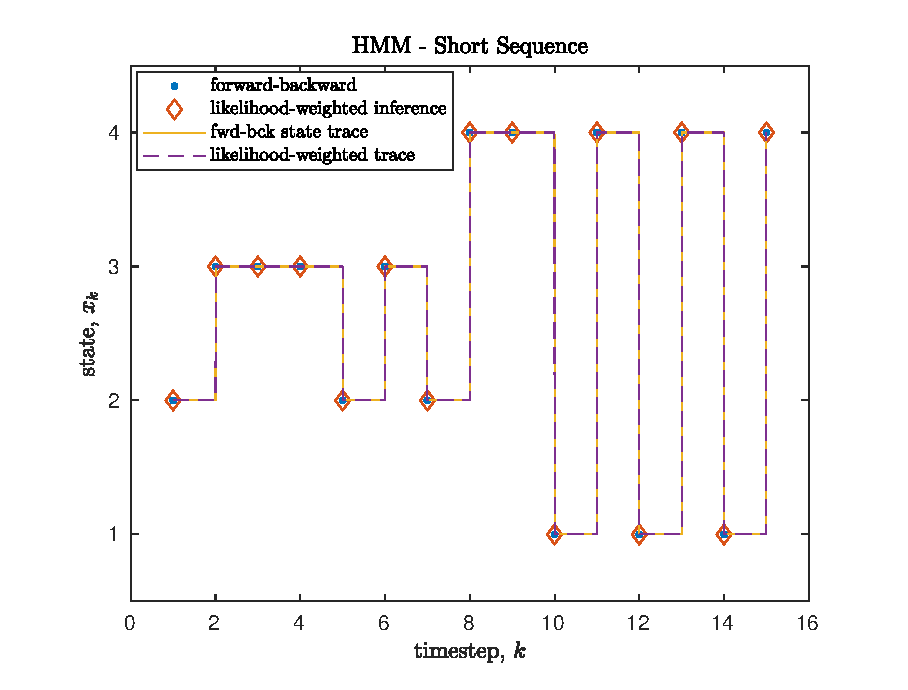
\includegraphics[scale=0.55]{p2_state_trace_1000_1.eps}  
			\caption{}
			\label{}
		\end{center}
	\end{subfigure}
	\hfill
	\begin{subfigure}[b]{0.45\textwidth}
		\begin{center}  
			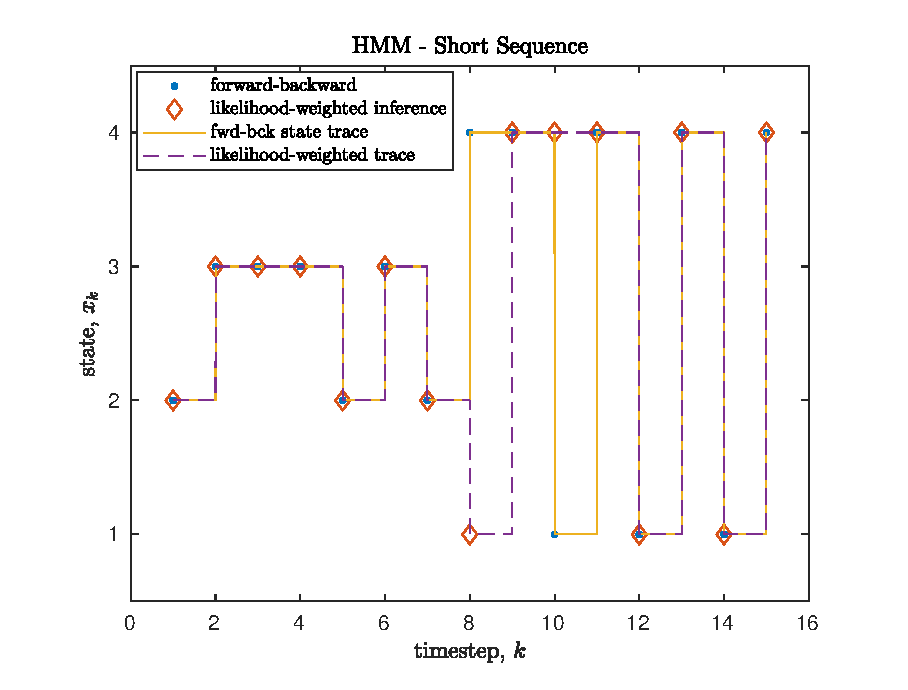
\includegraphics[scale=0.55]{p2_state_trace_1000_2.eps}  
			\caption{}
			\label{}
		\end{center}
	\end{subfigure}
	\caption{Monte Carlo sample size, $N_s$ = 1000}
\end{figure}

\begin{figure}[H]
	\begin{subfigure}[b]{0.45\textwidth}
		\begin{center}  
			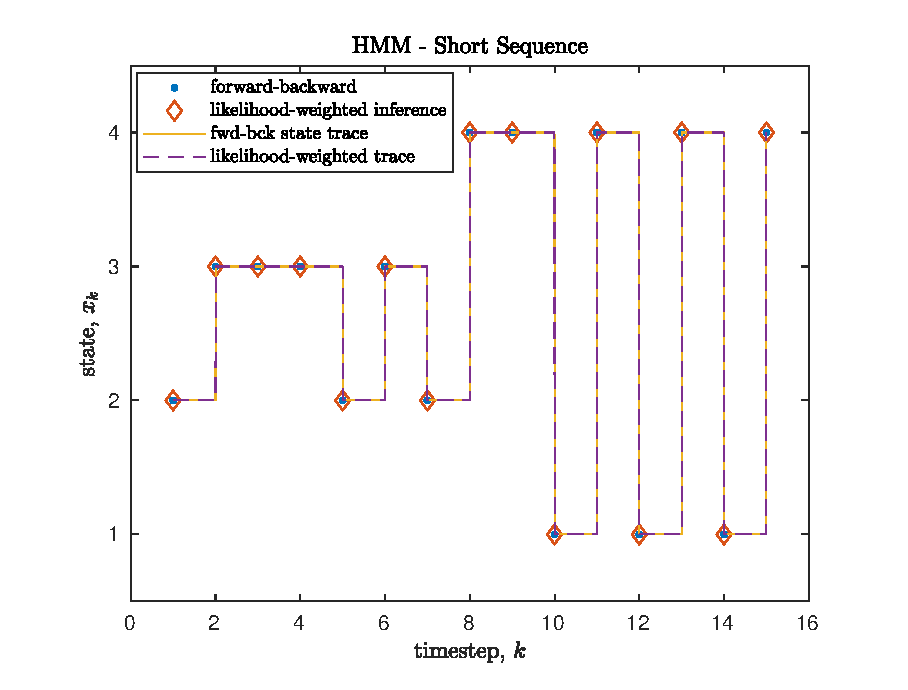
\includegraphics[scale=0.55]{p2_state_trace_10000_1.eps}  
			\caption{}
			\label{}
		\end{center}
	\end{subfigure}
	\hfill
	\begin{subfigure}[b]{0.45\textwidth}
		\begin{center}  
			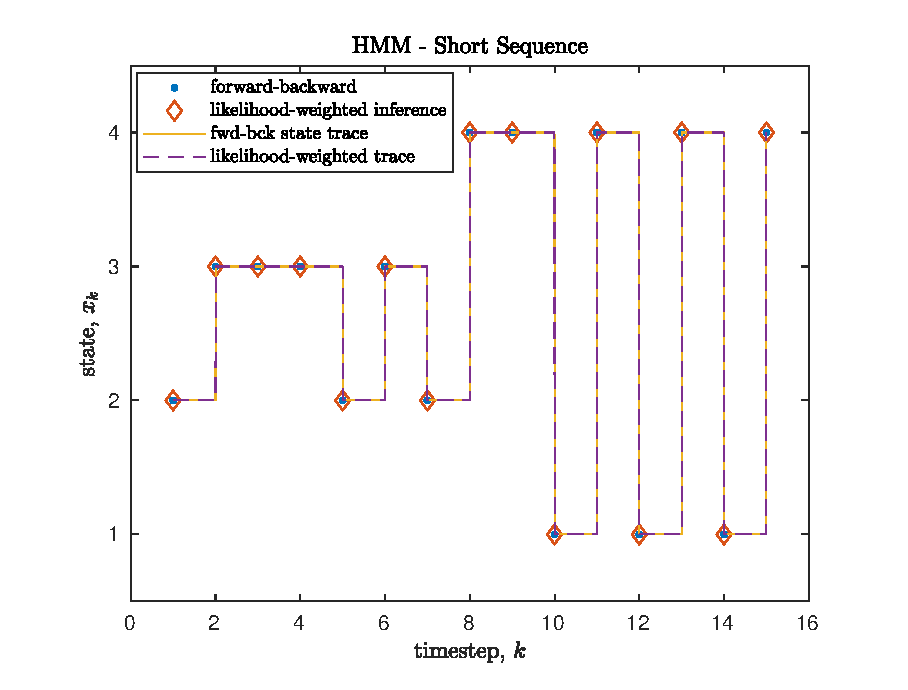
\includegraphics[scale=0.55]{p2_state_trace_10000_1.eps}  
			\caption{}
			\label{}
		\end{center}
	\end{subfigure}
	\caption{Monte Carlo sample size, $N_s$ = 10,000}
\end{figure}


\section*{Problem 3 - Mann Extended-Logarithm Forward-Backward Algorithm}
\addcontentsline{toc}{section}{Problem 3 - Mann Extended-Logarithm Forward-Backward Algorithm, Long Sequence}

Implement the forward-backward algorithm for the \texttt{nominal\_hmm\_long\_log.txt} sequence. Use the resulting posterior $P(x_k \vert y_{1:T})$ to classify the most likely state $x_k$ for each timestep $k=1:T$ (plot these as a time trace). In the state trace shown below, the states predicted by the standard Forward-Backward algorithm are compared against the states predicted by the Mann Extended-Logarithm Forward Backward algorithm.

\begin{figure}[H]
	\begin{center}  
		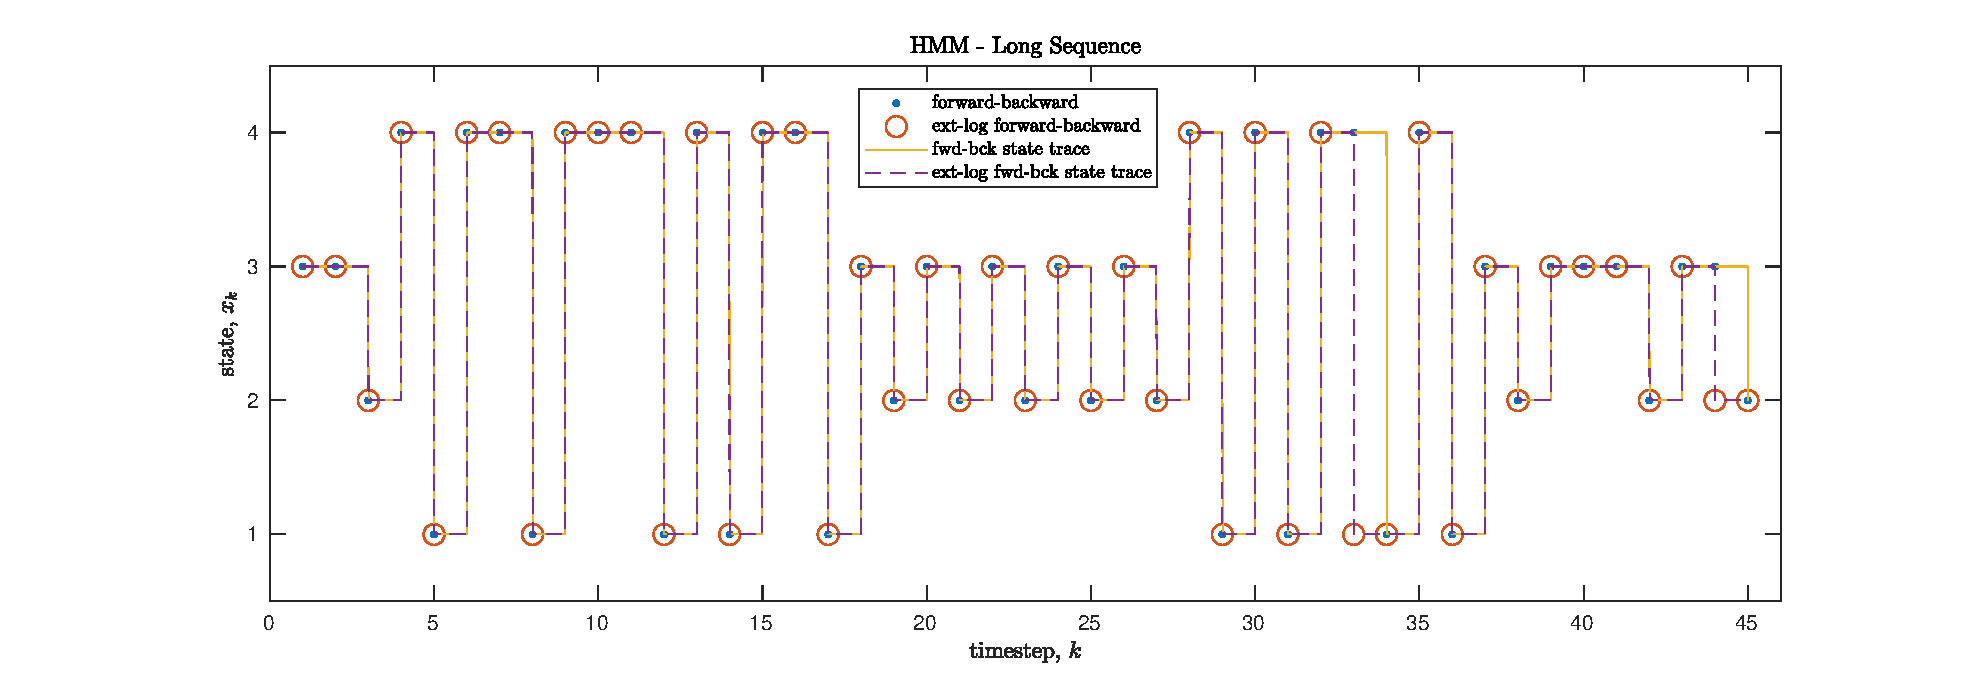
\includegraphics[scale=0.53]{p3_state_trace.eps}  
		\caption{Mann Extended-Logarithm Forward-Backward Algorithm state trace - Long Sequence}
		\label{fig:short_fb}
	\end{center}  
\end{figure}

Additionally, the data log-likelihood $\log P(y_{1:T})$, can be reported as follows:

\begin{equation}
	\log P(y_{1:T}) = \log \sum_{x_T} \alpha(x_T) = -84.743390
\end{equation}

\newpage
Report the posterior probabilities for only the first five and last five steps in the sequence.

\begin{table}[H]
	\caption{Forward-Backward Posterior Probabilities, $P(x_k \vert y_{1:T})$} 	% title of Table
	\centering 										% used for centering table
	\begin{tabular}{c c c c c} 						% centered columns (5 columns)
		\hline\hline 								%inserts double horizontal lines
		timestep, $k$ & $P(x_k = x_1 \vert y_{1:T})$ & $P(x_k = x_2 \vert y_{1:T})$ & $P(x_k = x_3 \vert y_{1:T})$ & $P(x_k = x_4 \vert y_{1:T})$ \\ [0.5ex] % inserts table
		%heading
		\hline 										% inserts single horizontal line
		1  & 0      & 0.1723 & 0.8277 & 0	   \\
		2  & 0      & 0.0058 & 0.9942 & 0      \\
		3  & 0      & 0.9951 & 0.0049 & 0      \\
		4  & 0.0062 & 0      & 0      & 0.9938 \\
		5  & 0.7125 & 0      & 0      & 0.2875 \\
		$\vdots$ &  &        &        &        \\
		41 & 0      & 0.0132 & 0.9868 & 0	   \\
		42 & 0      & 0.9435 & 0.0565 & 0      \\
		43 & 0      & 0.0134 & 0.9866 & 0      \\
		44 & 0      & 0.1575 & 0.8425 & 0      \\
		45 & 0      & 0.8313 & 0.1687 & 0      \\ [1ex]	% [1ex] adds vertical space							
		\hline 								% inserts single line
	\end{tabular}
	\label{table:posterior} 				% is used to refer this table in the text
\end{table}

The Tobias Mann Extended-Logarithm posterior probabilities are shown below for comparison.

\begin{table}[H]
	\caption{Mann Ext-Log Forward-Backward Posterior Probabilities, $P(x_k \vert y_{1:T})$} 	% title of Table
	\centering 										% used for centering table
	\begin{tabular}{c c c c c} 						% centered columns (5 columns)
		\hline\hline 								%inserts double horizontal lines
		timestep, $k$ & $P(x_k = x_1 \vert y_{1:T})$ & $P(x_k = x_2 \vert y_{1:T})$ & $P(x_k = x_3 \vert y_{1:T})$ & $P(x_k = x_4 \vert y_{1:T})$ \\ [0.5ex] % inserts table
		%heading
		\hline 										% inserts single horizontal line
		1  & 0      & 0.1404 & 0.8569 & 0	   \\
		2  & 0      & 0.0838 & 0.9162 & 0      \\
		3  & 0      & 0.9553 & 0.0447 & 0      \\
		4  & 0.0087 & 0      & 0      & 0.9913 \\
		5  & 0.9279 & 0      & 0      & 0.0721 \\
		$\vdots$ &  &        &        &        \\
		41 & 0      & 0.0699 & 0.9301 & 0	   \\
		42 & 0      & 0.9317 & 0.0683 & 0      \\
		43 & 0      & 0.0097 & 0.9903 & 0      \\
		44 & 0      & 0.5034 & 0.4966 & 0      \\
		45 & 0      & 0.8313 & 0.1687 & 0      \\ [1ex]	% [1ex] adds vertical space							
		\hline 								% inserts single line
	\end{tabular}
	\label{table:posterior} 				% is used to refer this table in the text
\end{table}

\newpage
\section*{Appendix - MATLAB Code}
\addcontentsline{toc}{section}{Appendix - MATLAB Code}

The following MATLAB code was used to generate the data presented above.\\

\textbf{hw1\_hmm.m} - main script
\begin{lstlisting}
%% Header

% Author: 		Carl Stahoviak
% Date Created:	2/19/2019

clc;
clear;
close ALL;

%% Load data

load('nominal_hmm_params.mat')

trans_prob = pxk_xkm1;
obs_prob = pyk_xk;

%% The Forward-Backward Algorithm (+ Ext-Log FB Alg.)

load('nominal_hmm_short_log.mat')
% load('nominal_hmm_long_log.mat')

%%% standard forward-backward algorithm
[alpha, alpha2] = forward( px0, trans_prob, obs_prob, y_obs );    % Txn
[beta, beta2] = backward( trans_prob, obs_prob, y_obs );          % Txn
% get the posterior distribution
posterior = fb_posterior( alpha(2:end,:)', beta' );               % Txn
[~,idx] = max(posterior');

% calculate data log-likelihood for forward-backward alg.
data_ll_fb = log(sum(alpha(end,:)));
fprintf('\nFB data log-likelihood = %f\n\n', data_ll_fb);

%%% Mann log-weighted (numerically-stable) forward-backward alg.
eln_alpha = forward_eln( px0, trans_prob, obs_prob, y_obs );
eln_beta = backward_eln( trans_prob, obs_prob, y_obs );
% get the posterior distribution
eln_posterior = elnfb_posterior( eln_alpha(2:end,:)', eln_beta' );
[~,eln_idx] = max(eln_posterior');

% calculate data log-likelihood for ext-log forward-backward alg.
data_ll_elnfb = nansum(nansum(eln_alpha,2));
fprintf('\nExt-Log FB data log-likelihood = %f\n\n', data_ll_elnfb);

%% Liklihood-Weighted Sampling

n = size(px0,1);    % number of states
Ns = 10000;         % number of Monte Carlo sample sequences

% get Ns Monte Carlo sample sequences of length T, and 
% corresponding sequence weights
T = size(y_obs,1);
[ lw_samples, weights ] = lw_sampling( Ns, T, px0, trans_prob, ...
obs_prob, y_obs);

% get likelihood-weighted (approximate?) inference posterior
lw_posterior = lw_inference( n, lw_samples, weights );
[~,lw_idx] = max(lw_posterior');

%% Plot Data

% create timeseries
t = linspace(1,size(y_obs,1),5000)';

% create empty continuous state vectors
state     = zeros(size(t,1),1);
eln_state = zeros(size(t,1),1);
lw_state  = zeros(size(t,1),1);

% create plot-friendly continuous states
for i=1:length(t)
state(i,1)     = idx(floor(t(i)));
eln_state(i,1) = eln_idx(floor(t(i)));
lw_state(i,1)  = lw_idx(floor(t(i)));
end

figure(1)
plot(idx,'.','MarkerSize',10); hold on;
plot(eln_idx,'o','MarkerSize',10);
plot(lw_idx,'diamond','MarkerSize',7);
plot(t,state);
plot(t,eln_state,'--');
% plot(t,lw_state,'--');
xlim([0,size(y_obs,1)+1])
ylim([0.5,4.5]); yticks([1 2 3 4 5])
title('HMM - Long Sequence','Interpreter','latex');
xlabel('timestep, $k$','Interpreter','latex');
ylabel('state, $x_k$','Interpreter','latex');
hdl = legend('forward-backward','ext-log forward-backward', ...
'likelihood-weighted inference','fwd-bck state trace', ...
'ext-log fwd-bck state trace');
set(hdl,'Interpreter','latex','Location','Northwest')
\end{lstlisting}

\textbf{forward.m} - forward pass of the forward-backward algorithm
\begin{lstlisting}
function [ alpha, alpha2 ] = forward( px0, trans_prob, obs_prob, y_obs )

n = size(px0,1);
T = size(y_obs,1);

% initialization - alpha(x0) = prior
alpha = zeros(n,T+1);
alpha(:,1) = px0;

alpha2 = zeros(n,T+1);
alpha2(:,1) = px0;

% forward pass
for k=1:T
	% matrix math version... works!
	alpha2(:,k+1) = alpha2(:,k)'*trans_prob'*diag(obs_prob(y_obs(k),:));
	for i=1:n
		for j=1:n
			alpha(i,k+1) = alpha(i,k+1) + ( alpha(j,k) * ...
				trans_prob(i,j) * obs_prob(y_obs(k),i) );
		end
	end
	% normalize (do NOT normalize alpha values!)
	% alpha(:,k+1) = alpha(:,k+1)./sum(alpha(:,k+1));
end

% return alpha with dmensions Txn
alpha = alpha';
alpha2 = alpha2';

end
\end{lstlisting}

\newpage
\textbf{backward.m} - backward pass of the forward-backward algorithm
\begin{lstlisting}
function [ beta, beta2 ] = backward( trans_prob, obs_prob, y_obs )

n = size(trans_prob,1);
T = size(y_obs,1);

% initialization
beta = zeros(n,T);
beta(:,end) = ones(n,1);

beta2 = zeros(n,T);
beta2(:,end) = ones(n,1);

% backward pass
for k=(T-1):-1:1
	% matrix math version... not working
	% beta2(:,k) = beta2(:,k+1)'*trans_prob*diag(obs_prob(y_obs(k+1),:));
	beta2(:,k) = obs_prob(y_obs(k+1),:)*trans_prob*diag(beta2(:,k+1));
	
	for i=1:n
		for j=1:n
			beta(i,k) = beta(i,k) + ( beta(j,k+1) * ...
				trans_prob(j,i) * obs_prob(y_obs(k+1),j) );
		end
	end
	% normalize (do NOT normalize beta values!)
	% beta(:,k) = beta(:,k)./sum(beta(:,k));
end

% return beta with dimensions Txn
beta = beta';
beta2 = beta2';

end
\end{lstlisting}

\textbf{fb\_posterior.m} - forward-backward algorithm posterior calculation
\begin{lstlisting}
function [ posterior ] = fb_posterior( alpha, beta )

if size(alpha,2) ~= size(beta,2)
	error('alpha, beta size mismatch')

else
	n = size(alpha,1);
	T = size(alpha,2);
	posterior = zeros(n,T);
	
	for k=1:T
		% sanity check
		fprintf('sum(alpha(:,%d).*beta(:,%d)) = %e\n', k, ...
			k, sum(alpha(:,k).*beta(:,k)))
		
		posterior(:,k) = (alpha(:,k).*beta(:,k)) / ...
		sum( alpha(:,k).*beta(:,k) );
		
		% normalize
		posterior(:,k) = posterior(:,k)./sum(posterior(:,k));
	end
	
	% return a Txn matrix
	posterior = posterior';
end
\end{lstlisting}
\newpage

\textbf{forward\_eln.m} - extended-logarithm forward pass
\begin{lstlisting}
function [ eln_alpha ] = forward_eln( px0, trans_prob, obs_prob, y_obs )

% use Mann notation
trans_prob = trans_prob';

n = size(px0,1);
T = size(y_obs,1);
eln_alpha = zeros(n,T+1);

% initialization
for i=1:n    
	% eln_alpha(i,1) = elnprod( eln(px0(i,1)), ...
	% 	eln(obs_prob(y_obs(1),i)) );
	eln_alpha(i,1) = eln(px0(i,1));
end

for k=2:T+1
	for j=1:n
		logalpha = NaN;
		for i=1:n 
			logalpha = elnsum( logalpha, ...
				elnprod( eln_alpha(i,k-1), eln(trans_prob(i,j)) ));
		end
		eln_alpha(j,k) = elnprod( logalpha, ...
			eln(obs_prob(y_obs(k-1),j)) );
	end
end

% return a Txn matrix
eln_alpha = eln_alpha';

end
\end{lstlisting}

\textbf{backward\_eln.m} - extended-logarithm backward pass
\begin{lstlisting}
function [ eln_beta ] = backward_eln( trans_prob, obs_prob, y_obs )

% use Mann notation
trans_prob = trans_prob';

n = size(trans_prob,1);
T = size(y_obs,1);

% initialization
eln_beta = zeros(n,T);

for k=(T-1):-1:1
	for i=1:n
	logbeta = NaN;
	for j=1:n 
		logbeta = elnsum( logbeta, ...
			elnprod( eln(trans_prob(i,j)), ...
			elnprod( obs_prob(y_obs(k+1),j), eln_beta(j,k+1) )));
		end
	eln_beta(i,k) = logbeta;
	end
end

% return a Txn matrix
eln_beta = eln_beta';
\end{lstlisting}

\newpage
\textbf{elnfb\_posterior.m} - extended-logarithm posterior calculation
\begin{lstlisting}
function [ eln_post ] = elnfb_posterior( eln_alpha, eln_beta )

if size(eln_alpha,2) ~= size(eln_beta,2)
	error('eln_alpha, eln_beta size mismatch')

else
	n = size(eln_alpha,1);
	T = size(eln_alpha,2);
	
	eln_gamma = zeros(n,T);     % log-posterior
	gamma = zeros(n,T);         % true posterior
	
	for k=1:T
		normalizer = NaN;
		for i=1:n
			eln_gamma(i,k) = elnprod(eln_alpha(i,k),eln_beta(i,k));
			normalizer = elnsum(normalizer,eln_gamma(i,k));
		end
		
		for i=1:n
			eln_gamma(i,k) = elnprod(eln_gamma(i,k),-normalizer);
			gamma(i,k) = eexp(eln_gamma(i,k));
		end
		% sanity check
		fprintf('1 - sum(gamma(:,%d)) = %e\n', k, 1-sum(gamma(:,k))) 
	end
end

% return a Txn matrix
eln_post = gamma';;
\end{lstlisting}

\textbf{lw\_sampling.m} - likelihood-weighted sampling
\begin{lstlisting}
function [ lw_samples, weights ] = lw_sampling( Ns, T, px0, trans_prob, obs_prob, y_obs )
%LW_SAMPLING Liklihood Weighted Sampling

lw_samples = zeros(Ns,T);   % V_E - likelihood weighted sample
weights = ones(Ns,1);       % W_E - likelihood weights

% get intial state from prior distribution, px0
[~,idx] = max(px0);

for s=1:Ns
	for k=1:T
	if k==1
		% draw random sample according to initial (known) state, x0
		lw_samples(s,k) = randsample(4,1,true, trans_prob(:,idx)); 
	else
		% draw random sample according to state transtion probabilities
		lw_samples(s,k) = randsample(4,1,true, trans_prob(:,lw_samples(s,k-1))); 
	end
	
	% update sequence weight:
	% weight = weight * P( y_k | Pa(y_k) = x_k )
	% NOTE: parent of each observation y_k is the state x_k
	weights(s,1) = weights(s,1) * obs_prob(y_obs(k),lw_samples(s,k));
	end
end

end

\end{lstlisting}

\newpage
\textbf{lw\_inference.m} - likelihood-weighted approximate inference
\begin{lstlisting}
function [ posterior ] = lw_inference( n, lw_samples, weights )
%LW_INFERENCE Likelihood-weighted approximate inference

T = size(lw_samples,2);
posterior = zeros(n,T);

for k=1:T
	for i=1:n
	% get index location of where x_k = x_i across all sequences
	idx = (lw_samples(:,k) == i);
	
	% the posterior for each state i at timestep k is the weighted sum
	% of the relaizations (indicator function) of state x_i at
	% timestep k across all MC sample sequences
	posterior(i,k) = sum(weights(idx))/sum(weights);
	end
end

posterior = posterior';

end

\end{lstlisting}

Mann Extended-Logarithm Functions Library
\begin{lstlisting}
function [ out ] = eexp( x )
% EEXP - Extended Exponential function

	% if x == 'LOGZERO'
	if isnan(x)
		out = 0;
	else
		out = exp(x);
	end

end

function [ out ] = eln( x )
% ELN - Extended Natural Logarathm function
%   Computes the extended natural logarithm as defined by Mann, 2006

	if x == 0
		% out = 'LOGZERO';
		out = NaN;
	elseif x > 0
		out = log(x);
	else
		error('eln() negative input error')   
	end

end

function [ prod ] = elnprod( eln_x, eln_y )
% ELNSUM - Extended Logartithm Product function
%   Computes the extended logarithm of the product of x and y given as
%   given as inputs the extended logarithm of x and y, as defined by Mann, 2006

	% if strcmp(eln(x),'LOGZERO') || strcmp(eln(y),'LOGZERO')
	if isnan(eln_x) || isnan(eln_y)
		% prod = 'LOGZERO';
		prod = NaN;
	else
		prod = eln_x + eln_y;
	end

end

function [ sum ] = elnsum( eln_x, eln_y )
% ELNSUM - Extended Logartithm Sum function
%   Computes the extended logarithm of the sum of x and y given as inputs 
%   the extended logarithm of x and y, as defined by Mann, 2006

	% if strcmp(eln(x),'LOGZERO') || strcmp(eln(y),'LOGZERO')
	if isnan(eln_x) || isnan(eln_y)
		% if strcmp(eln(x),'LOGZERO')
		if isnan(eln_x)
			sum = eln_y;
		else
			sum = eln_x;
		end
	else
		if eln_x > eln_y
			sum = eln_x + eln(1 + exp(eln_y-eln_x));
		else
			sum = eln_y + eln(1 + exp(eln_x-eln_y));
		end
	end

end
\end{lstlisting}


\end{document}